\subsection{实验设置}

实验围绕四个问题组织。KCH-MedRank 比强基线（含生物医学交叉编码器）好多少？超图结构有帮助还是原始拓扑会引入噪声？收益能否泛化到 BioASQ 之外？重排序器在哪里成败？对应章节是主实验结果（第~\ref{sec:main-results} 节）、结构消融（第~\ref{sec:ablation} 节）、本节内的 PubMedQA 和 BEIR NFCorpus 稳健性诊断，以及可解释性和错误分析（第~\ref{sec:interpretability} 节）。

\subsubsection{数据集与划分}

主数据集为 \texttt{rag-datasets/rag-mini-bioasq}，包含 4,719 个 BioASQ 风格问题，带金标准段落级标注。我们按问题标识符模 5 分桶做确定性问题级划分：训练覆盖桶 0--2（2,832 个问题），验证用桶 3（944 个问题），测试用桶 4（943 个问题）。划分在所有模型选择之前固定。每个问题携带多条金标准证据段落，因此 Recall@$k$（宏证据覆盖率）是主要指标。

PubMedQA~\citep{jin2019pubmedqa} 以 yes/no/maybe 问答格式和强首位命中检索作为辅助诊断。BEIR NFCorpus~\citep{thakur2021beir} 是外部仅检索稳健性测试。MeSH、实体和超图特征未为 NFCorpus 构建，仅比较仅检索特征的 LambdaMART。

\subsubsection{基线}

第一阶段检索器包括 BM25、稠密生物医学检索、原始 Hybrid RRF（BM25 和稠密等权）、带 MeSH 扩展的 fielded BM25、MedCPT 双编码器检索，以及在验证集 Recall@100 上选取 w122 配置的增强 Hybrid RRF。

重排序基线从最强的可用语义模型一直到最简单的仅检索排序器：同一增强候选池上的 MedCPT Cross-Encoder~\citep{jin2023medcpt}、无生物医学知识的仅检索特征 LambdaMART、含所有知识特征但无图结构的扁平生物医学知识 LambdaMART、成对图 LTR、无医学知识超图 LTR、以及完整 KCH-MedRank。

\subsubsection{评估协议}

指标为 Recall@$k$、Hit@$k$、MRR@$k$ 和 nDCG@$k$，$k \in \{1,3,5,10,20,50,100\}$。Recall@$k$ 是宏证据覆盖率：每个问题 top $k$ 中金标准段落占该问题全部金标准段落的比例，对问题取平均。统计显著性来自成对 bootstrap，10,000 次重采样，固定随机种子。所有模型选择仅使用验证集指标，测试集仅评估一次。

困难重排序子集隔离了 65 个测试问题，其增强 Hybrid RRF 候选池 top 100 中含有金标准证据但 top 10 中没有一条金标准段落。此子集上基线 Recall@10 按构造为 0。通过它意味着知识特征救回了检索信号独自无法救回的证据。

\begin{table}[t]
\centering
\small
\caption{验证集选择的增强候选生成设置，融合权重仅在验证集上选择。}
\label{tab:enhanced-candidate-selection}
\begin{tabular}{lrrrrrr}
\toprule
融合设置 & BM25 & Dense & Fielded BM25 & MedCPT DE & 验证 R@100 & 测试 R@100 \\
\midrule
Original Hybrid & 1.0 & 1.0 & 0.0 & 0.0 & 0.6325 & 0.6077 \\
w052 & 1.0 & 1.0 & 0.5 & 0.2 & 0.6391 & 0.6163 \\
w084 & 1.0 & 1.0 & 0.8 & 0.4 & 0.7329 & 0.7084 \\
w102 & 1.0 & 1.0 & 1.0 & 0.2 & 0.7529 & 0.7285 \\
w122, selected & 1.0 & 1.0 & 1.2 & 0.2 & 0.7568 & 0.7388 \\
\bottomrule
\end{tabular}
\end{table}



\begin{figure}[htbp]
\centering
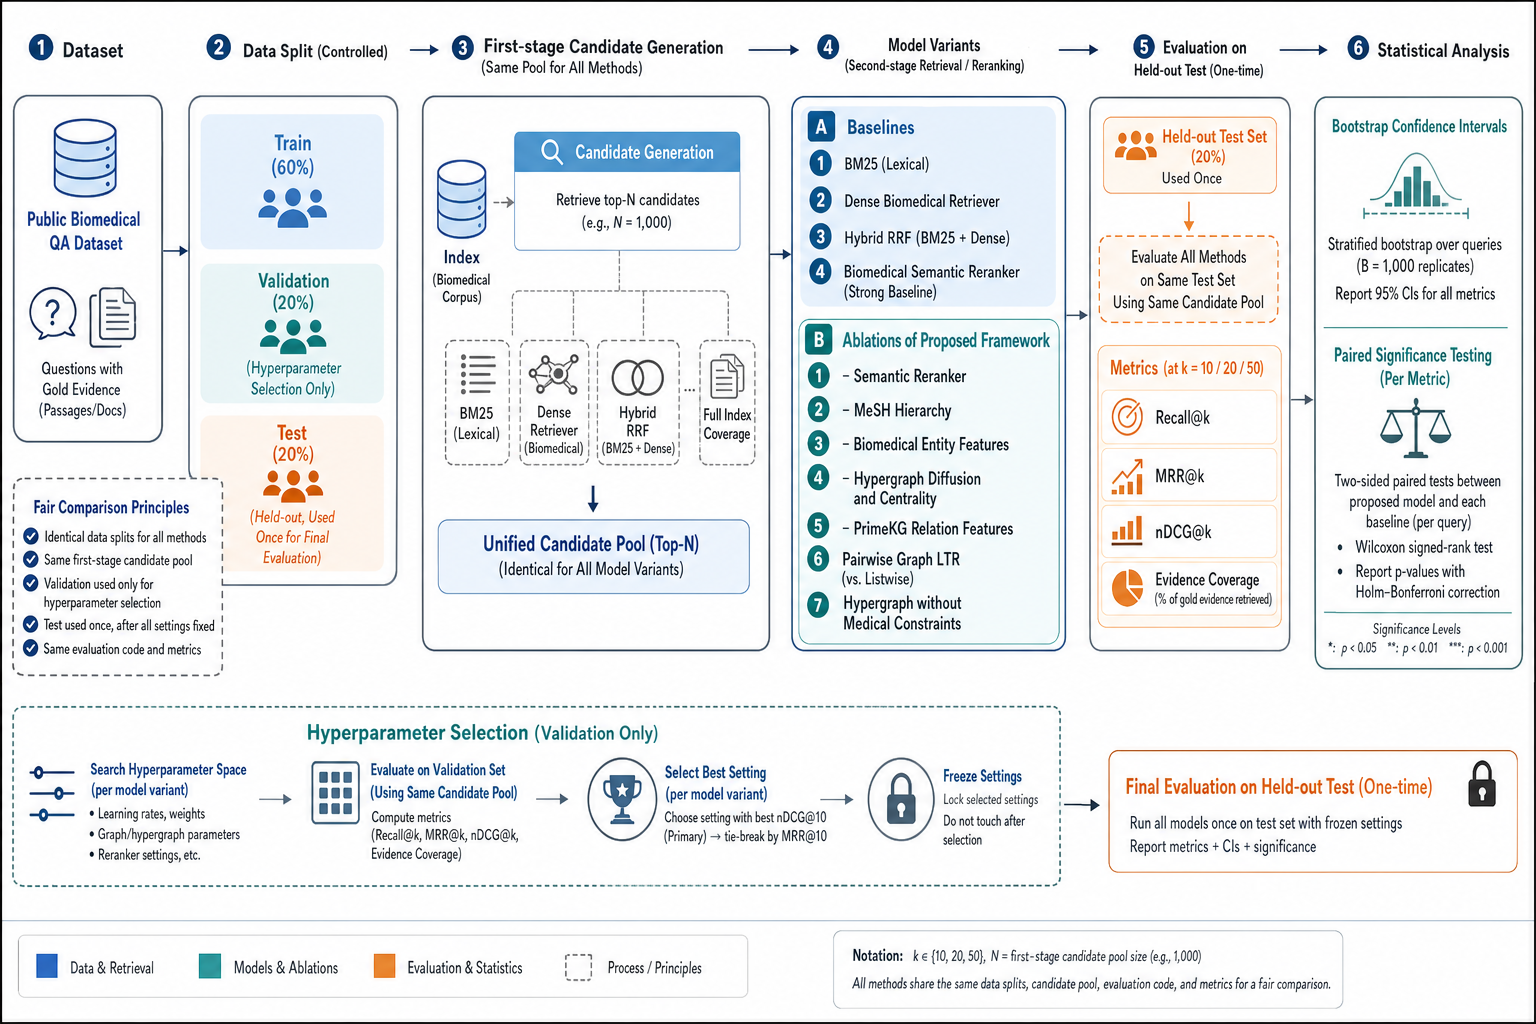
\includegraphics[width=0.98\linewidth]{figures/gpt_image2_figure_04.png}
\caption{受控实验设计：候选生成、重排序基线、结构消融、仅验证集模型选择和成对统计检验。}
\label{fig:gpt-experimental-design}
\end{figure}
